%!TEX root = ../../report.tex
\section{Monte Carlo Localization with Dynamic Map Representation}
\label{sec:amcl_dyn_map}
The effect of performing localization with AMCL on an updated map representation in the form of the costmap described in section \ref{sec:localzation_feature_map} is evaluated by comparing the estimated pose covariances with the ones achieved when using a static map representation. 
The sizes of the elements of the covariance matrix indicates the certainty of the estimated pose of the robot with respect to the map frame. 
Larger values is evidence for an uncertain pose estimation. Hence the estimated covariance do not indicate how accurate the location estimate is, but how widely spread the particles is. 
It can happen that AMCL is very certain on a wrong position. 

The test setup evaluates a situation where a mobile robot navigates in an area for some time, then it moves away and comes back to a changed environment and navigates there for the same amount of time. 
This is repeated for four times using both a static map representation and a map that is adapted to the changes using the Dynamic mapping system. 

\subsection{Industrial Test Environment}
The evaluation is performed on the MiR-100 robot with the software version 1.5.1. It was performed in Robolab at SDU, which is similar to an industrial environments. Initially the environment was mapped with the Hector SLAM algorithm contained in the MIR software. 
Afterwards, small obstacles which might be moved during the evaluation was removed.
The generated map is shown in figure \ref{fig:Robolab1_clean_with_cam}, where the approximate pose of the camera when taking the images shown in figure \ref{fig:robolab_mayhem} is indicated. 
The camera is positioned on the first floor and tilted.

\begin{figure}[tbph]
	\centering
	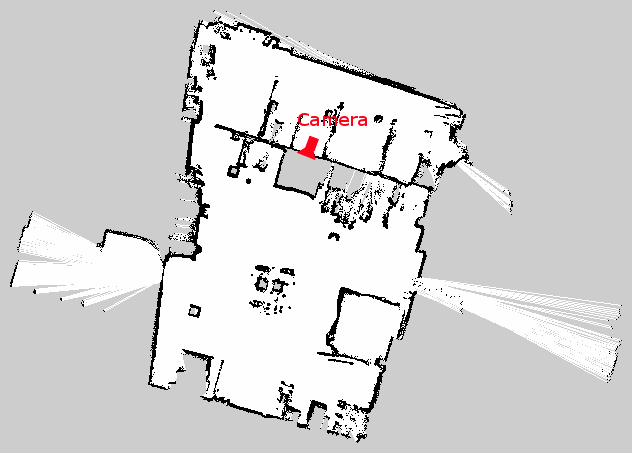
\includegraphics[width=0.7\linewidth]{chapters/evaluation/figures/Robolab1_clean_with_cam}
	\caption{The static map used by AMCL with indication of the camera's pose when taking the images in figure \ref{fig:robolab_mayhem}.}
	\label{fig:Robolab1_clean_with_cam}
\end{figure}

The test was performed by letting the robot navigate around the obstacles located central in the room continually for 25 minutes two times in four different environments. 
For each of the environments the robot performed localization on the static map in figure \ref{fig:Robolab1_clean_with_cam} and with a map constructed by the Dynamic mapping system for 25 minutes. 
The Dynamic mapping system incorporates the information collected in the previous test runs.
The first updated map is created using the data collected using the static map representation and the second also incorporates the data collected when localizing with the previous dynamic map. 
The third also incorporates the data collected in the previous experiment when localizing with a dynamic map and so on for the two consecutive environments.

\begin{figure}[htbp]
	\begin{subfigure}[t]{0.499\textwidth}	
		\centering	
		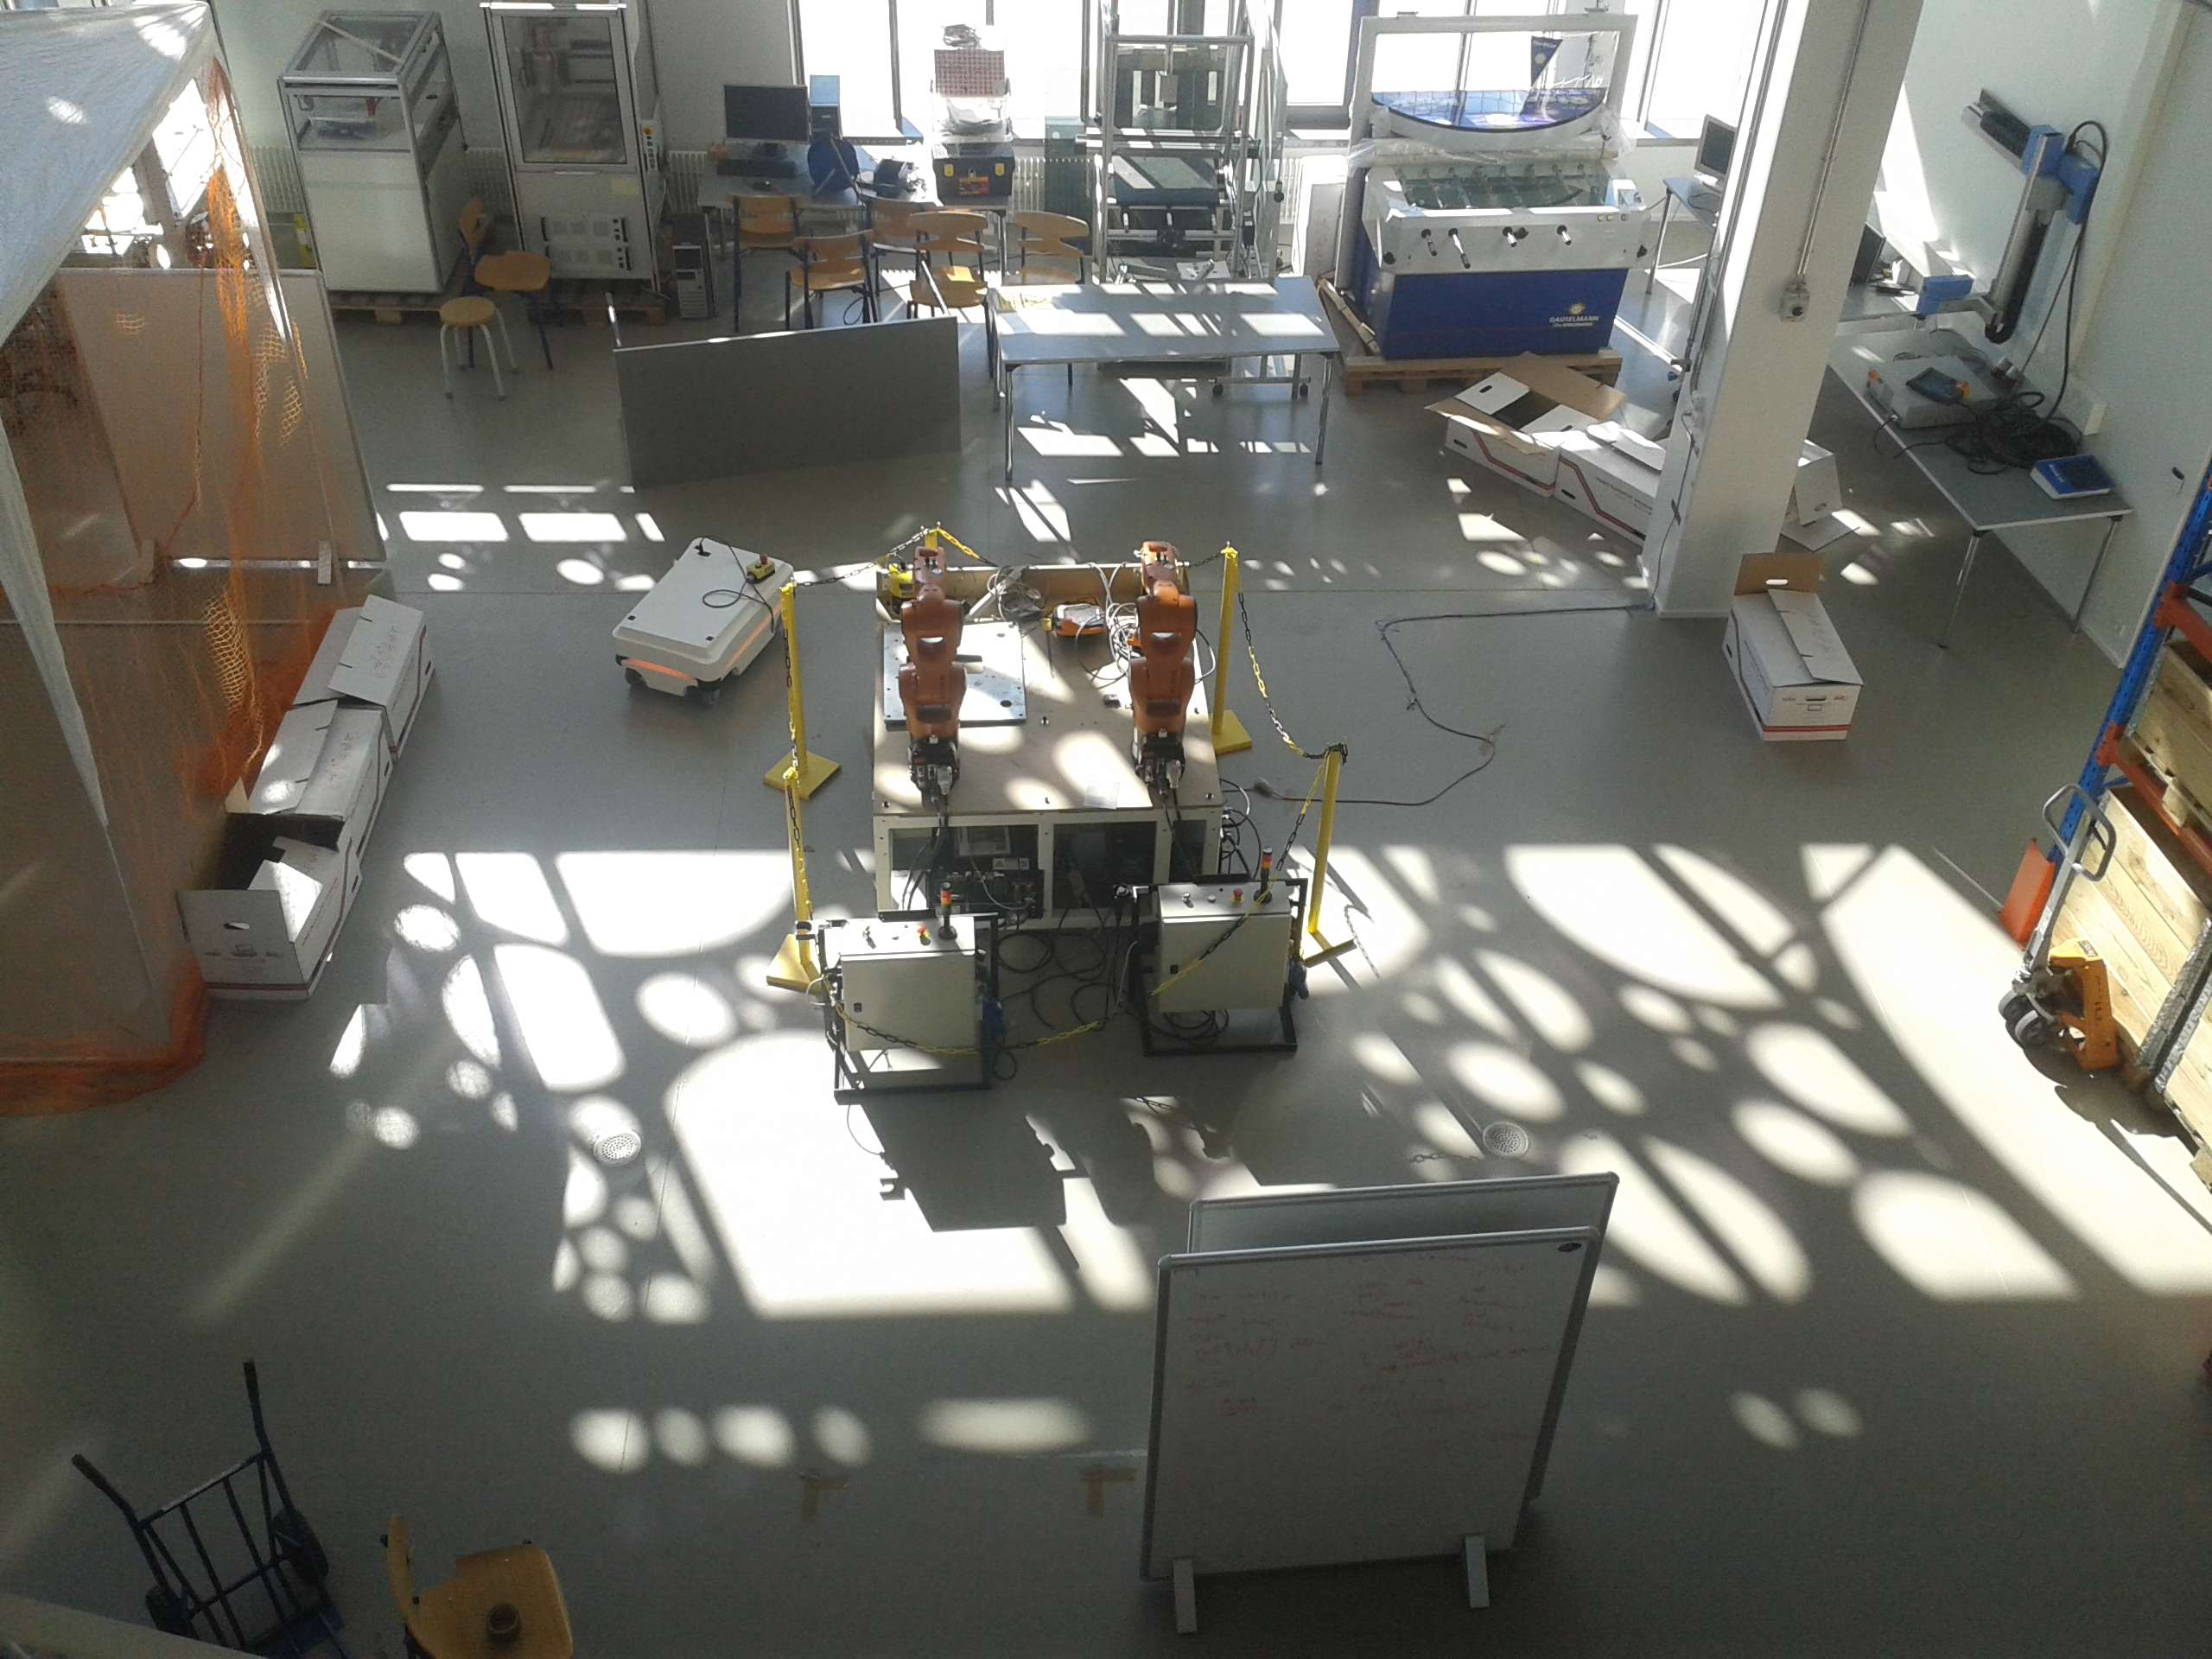
\includegraphics[width=1\textwidth]{chapters/evaluation/figures/mayhem_robolab1}
		\caption{First environment}
		\label{fig:location_environment1}
	\end{subfigure}
	\begin{subfigure}[t]{0.499\textwidth}
		\centering
		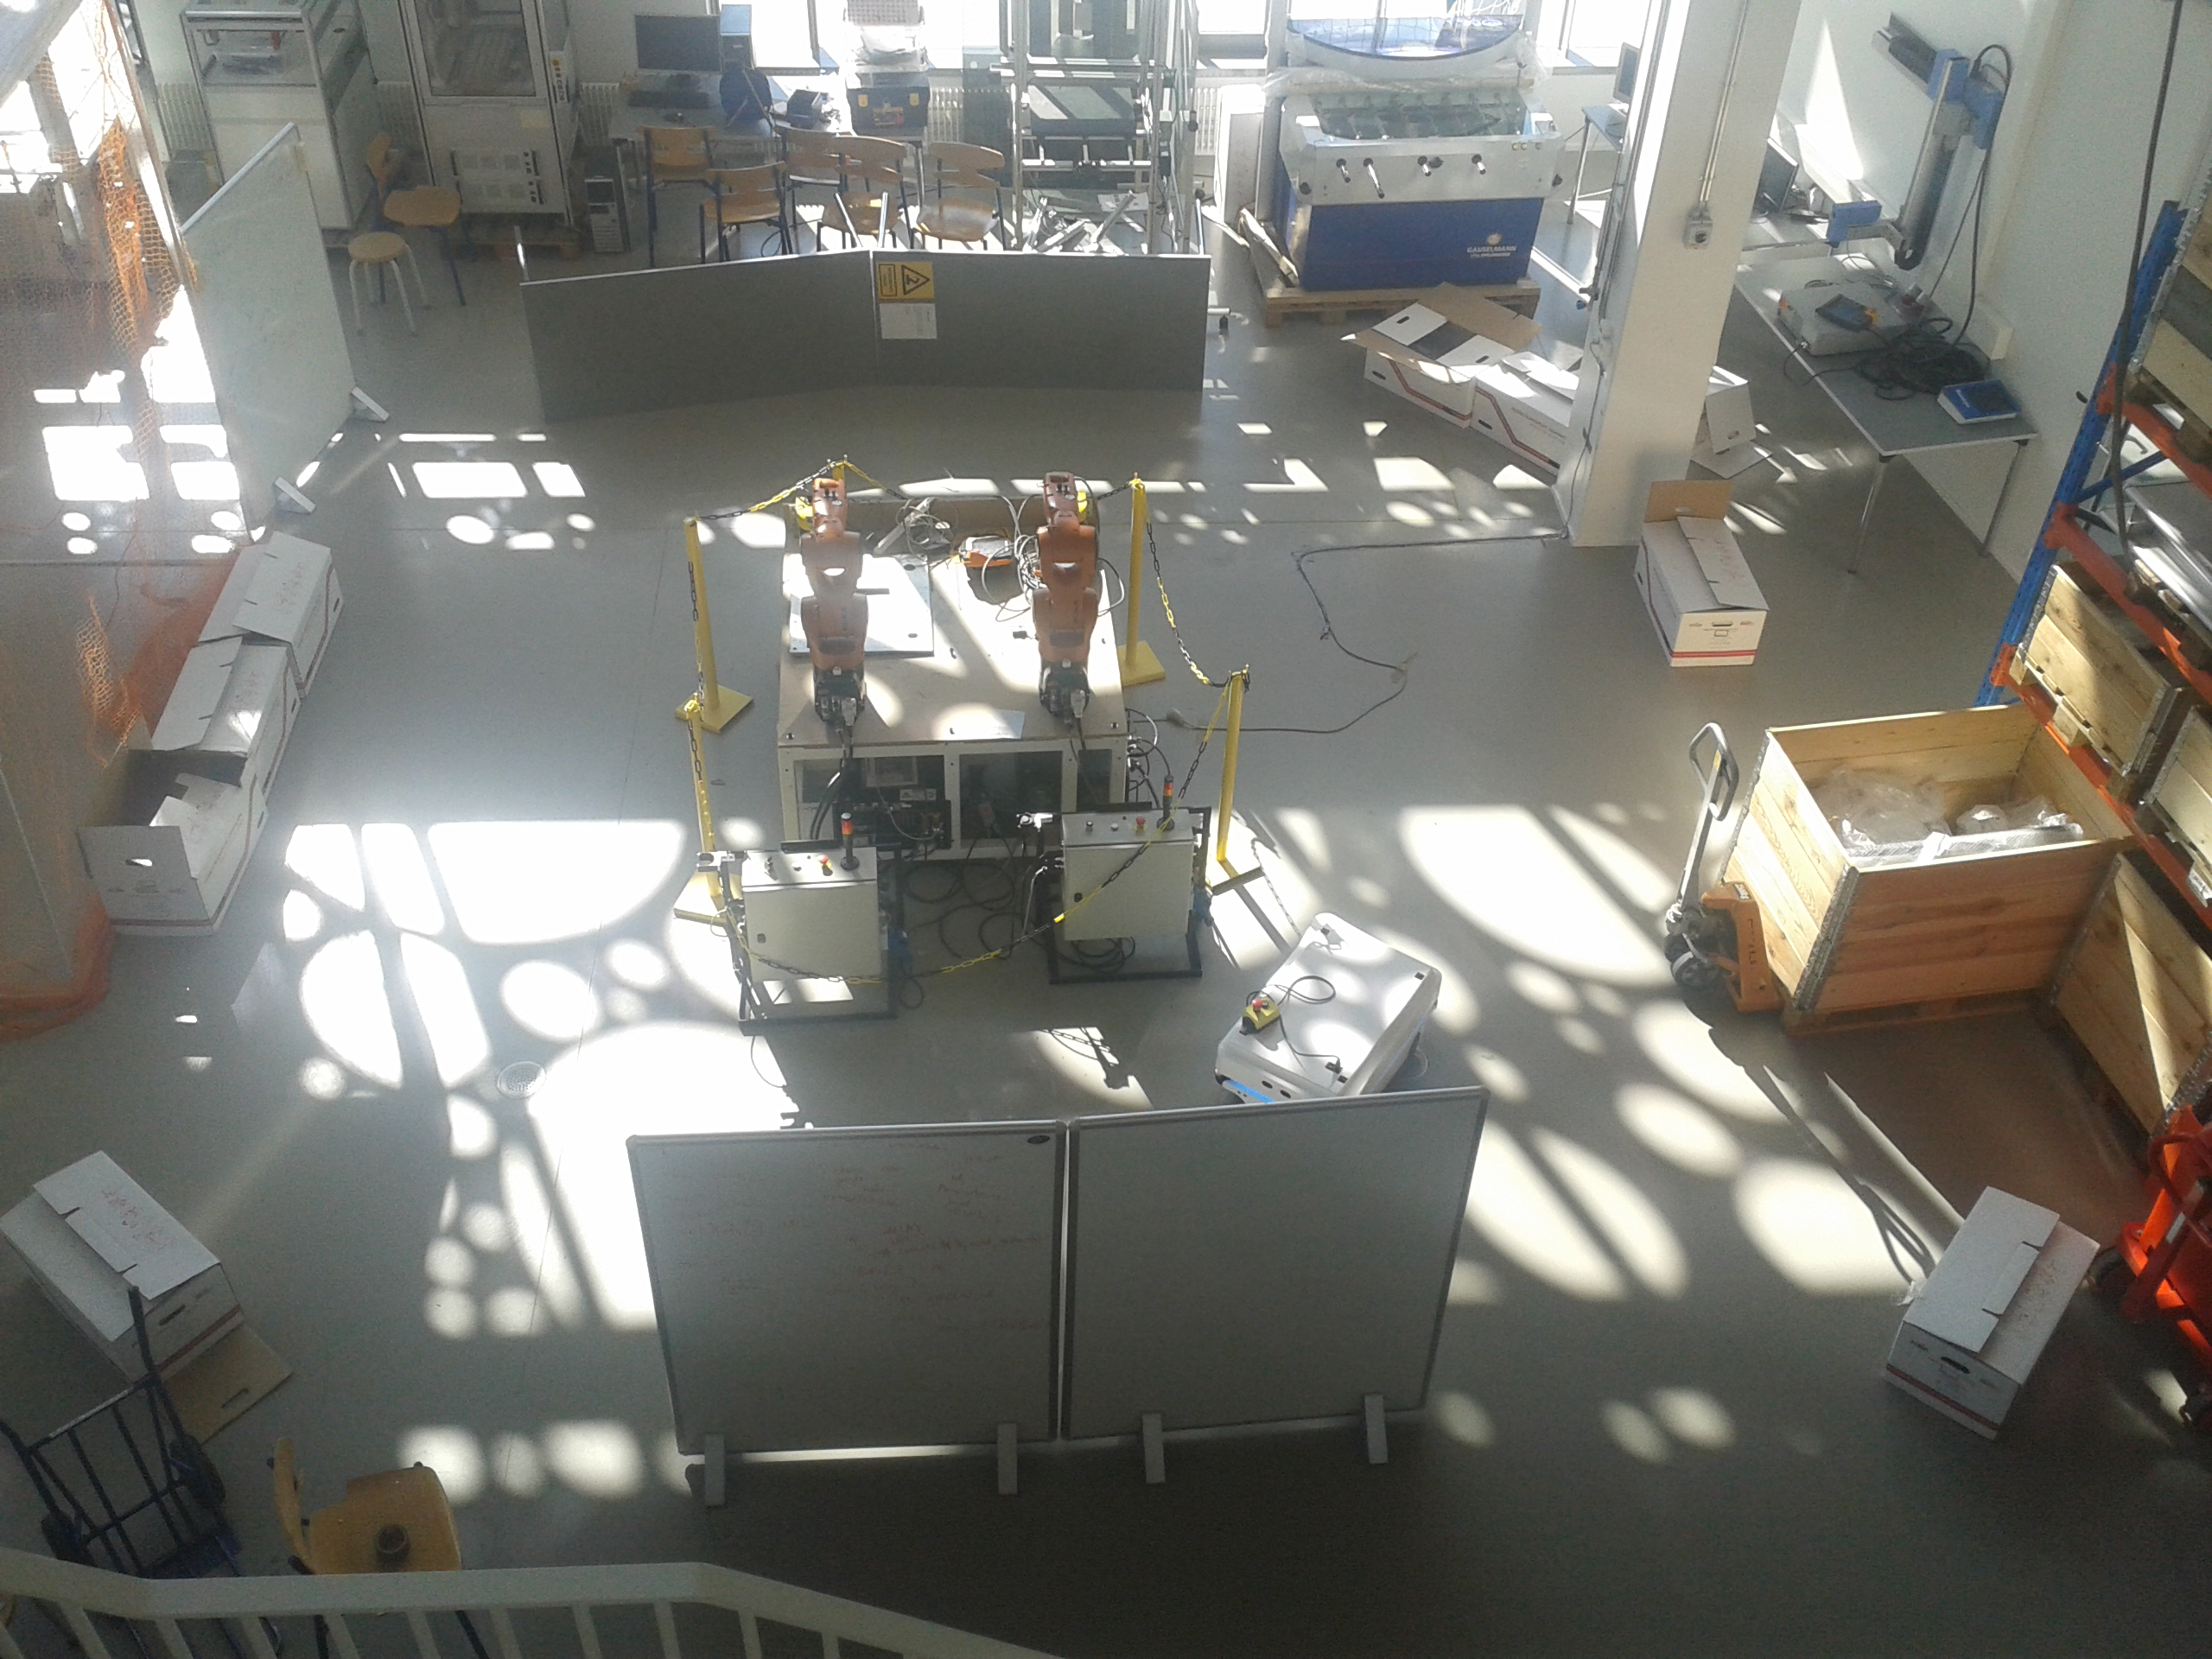
\includegraphics[width=1\textwidth]{chapters/evaluation/figures/mayhem_robolab2}
		\caption{Second environment}
		\label{fig:location_environment2}
	\end{subfigure}
	\begin{subfigure}[t]{0.499\textwidth}
		\centering
		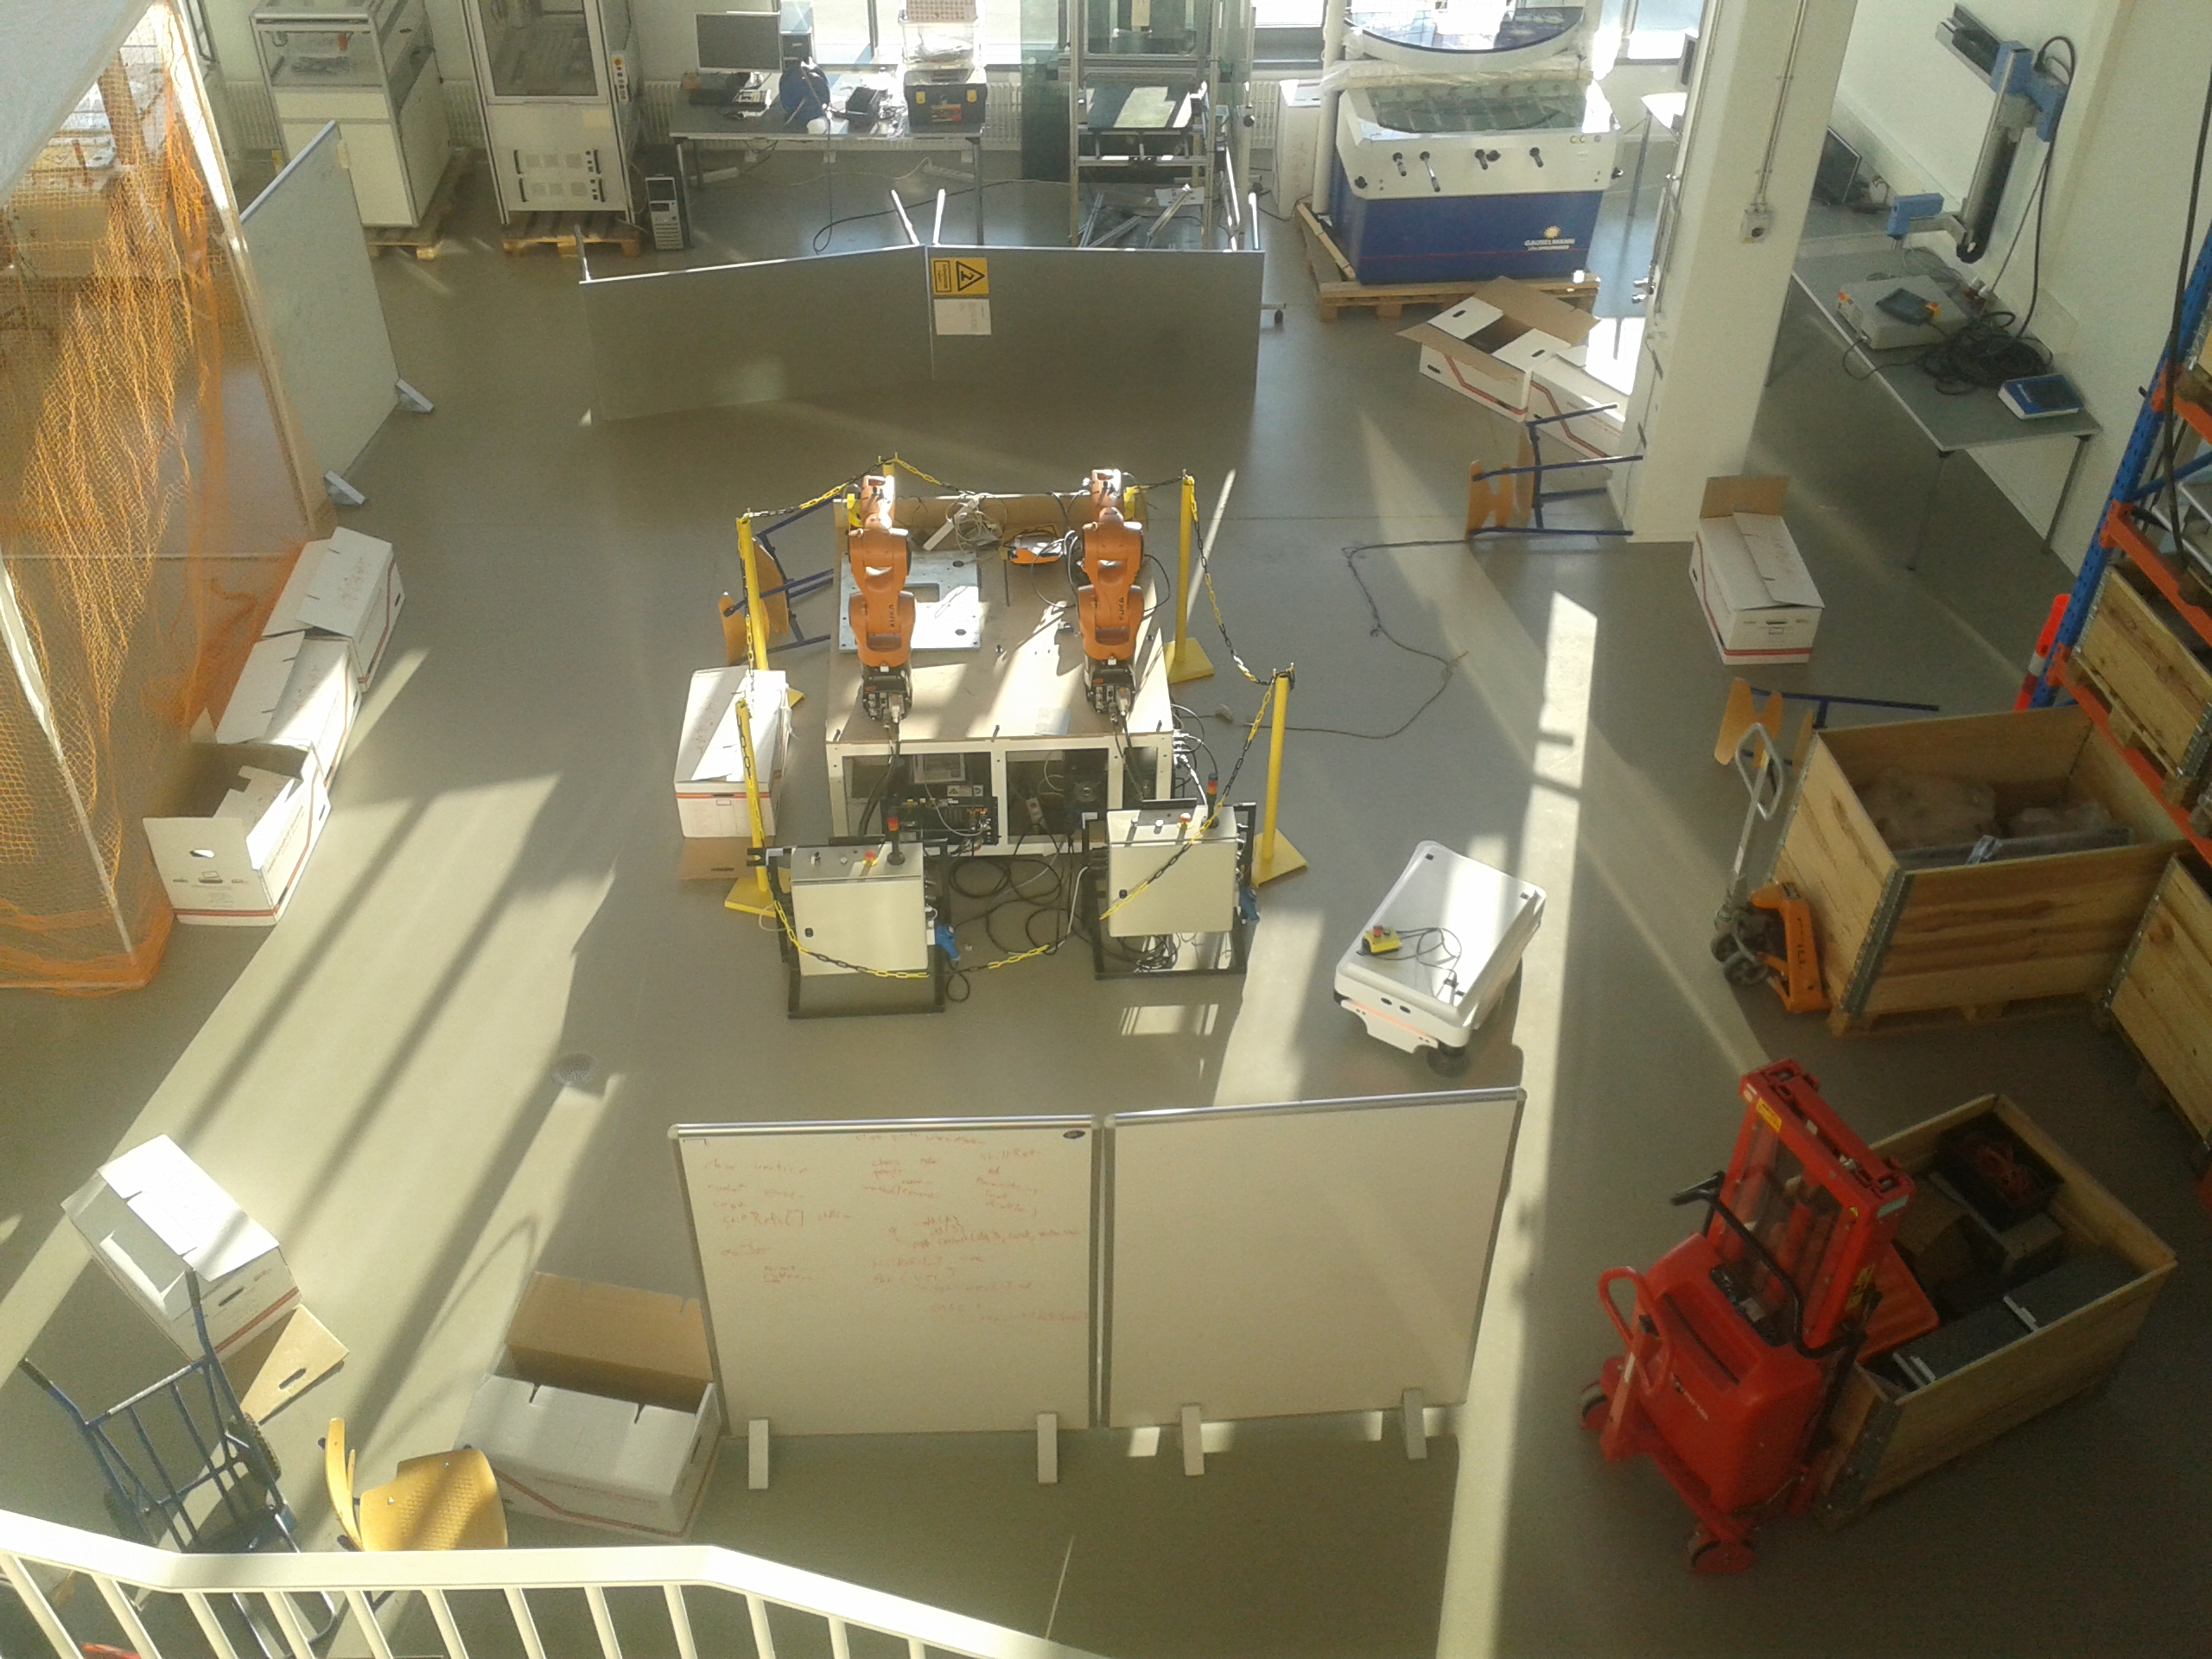
\includegraphics[width=1\textwidth]{chapters/evaluation/figures/mayhem_robolab3}
		\caption{Third environment}
		\label{fig:location_environment3}
	\end{subfigure}
	\begin{subfigure}[t]{0.499\textwidth}
		\centering
		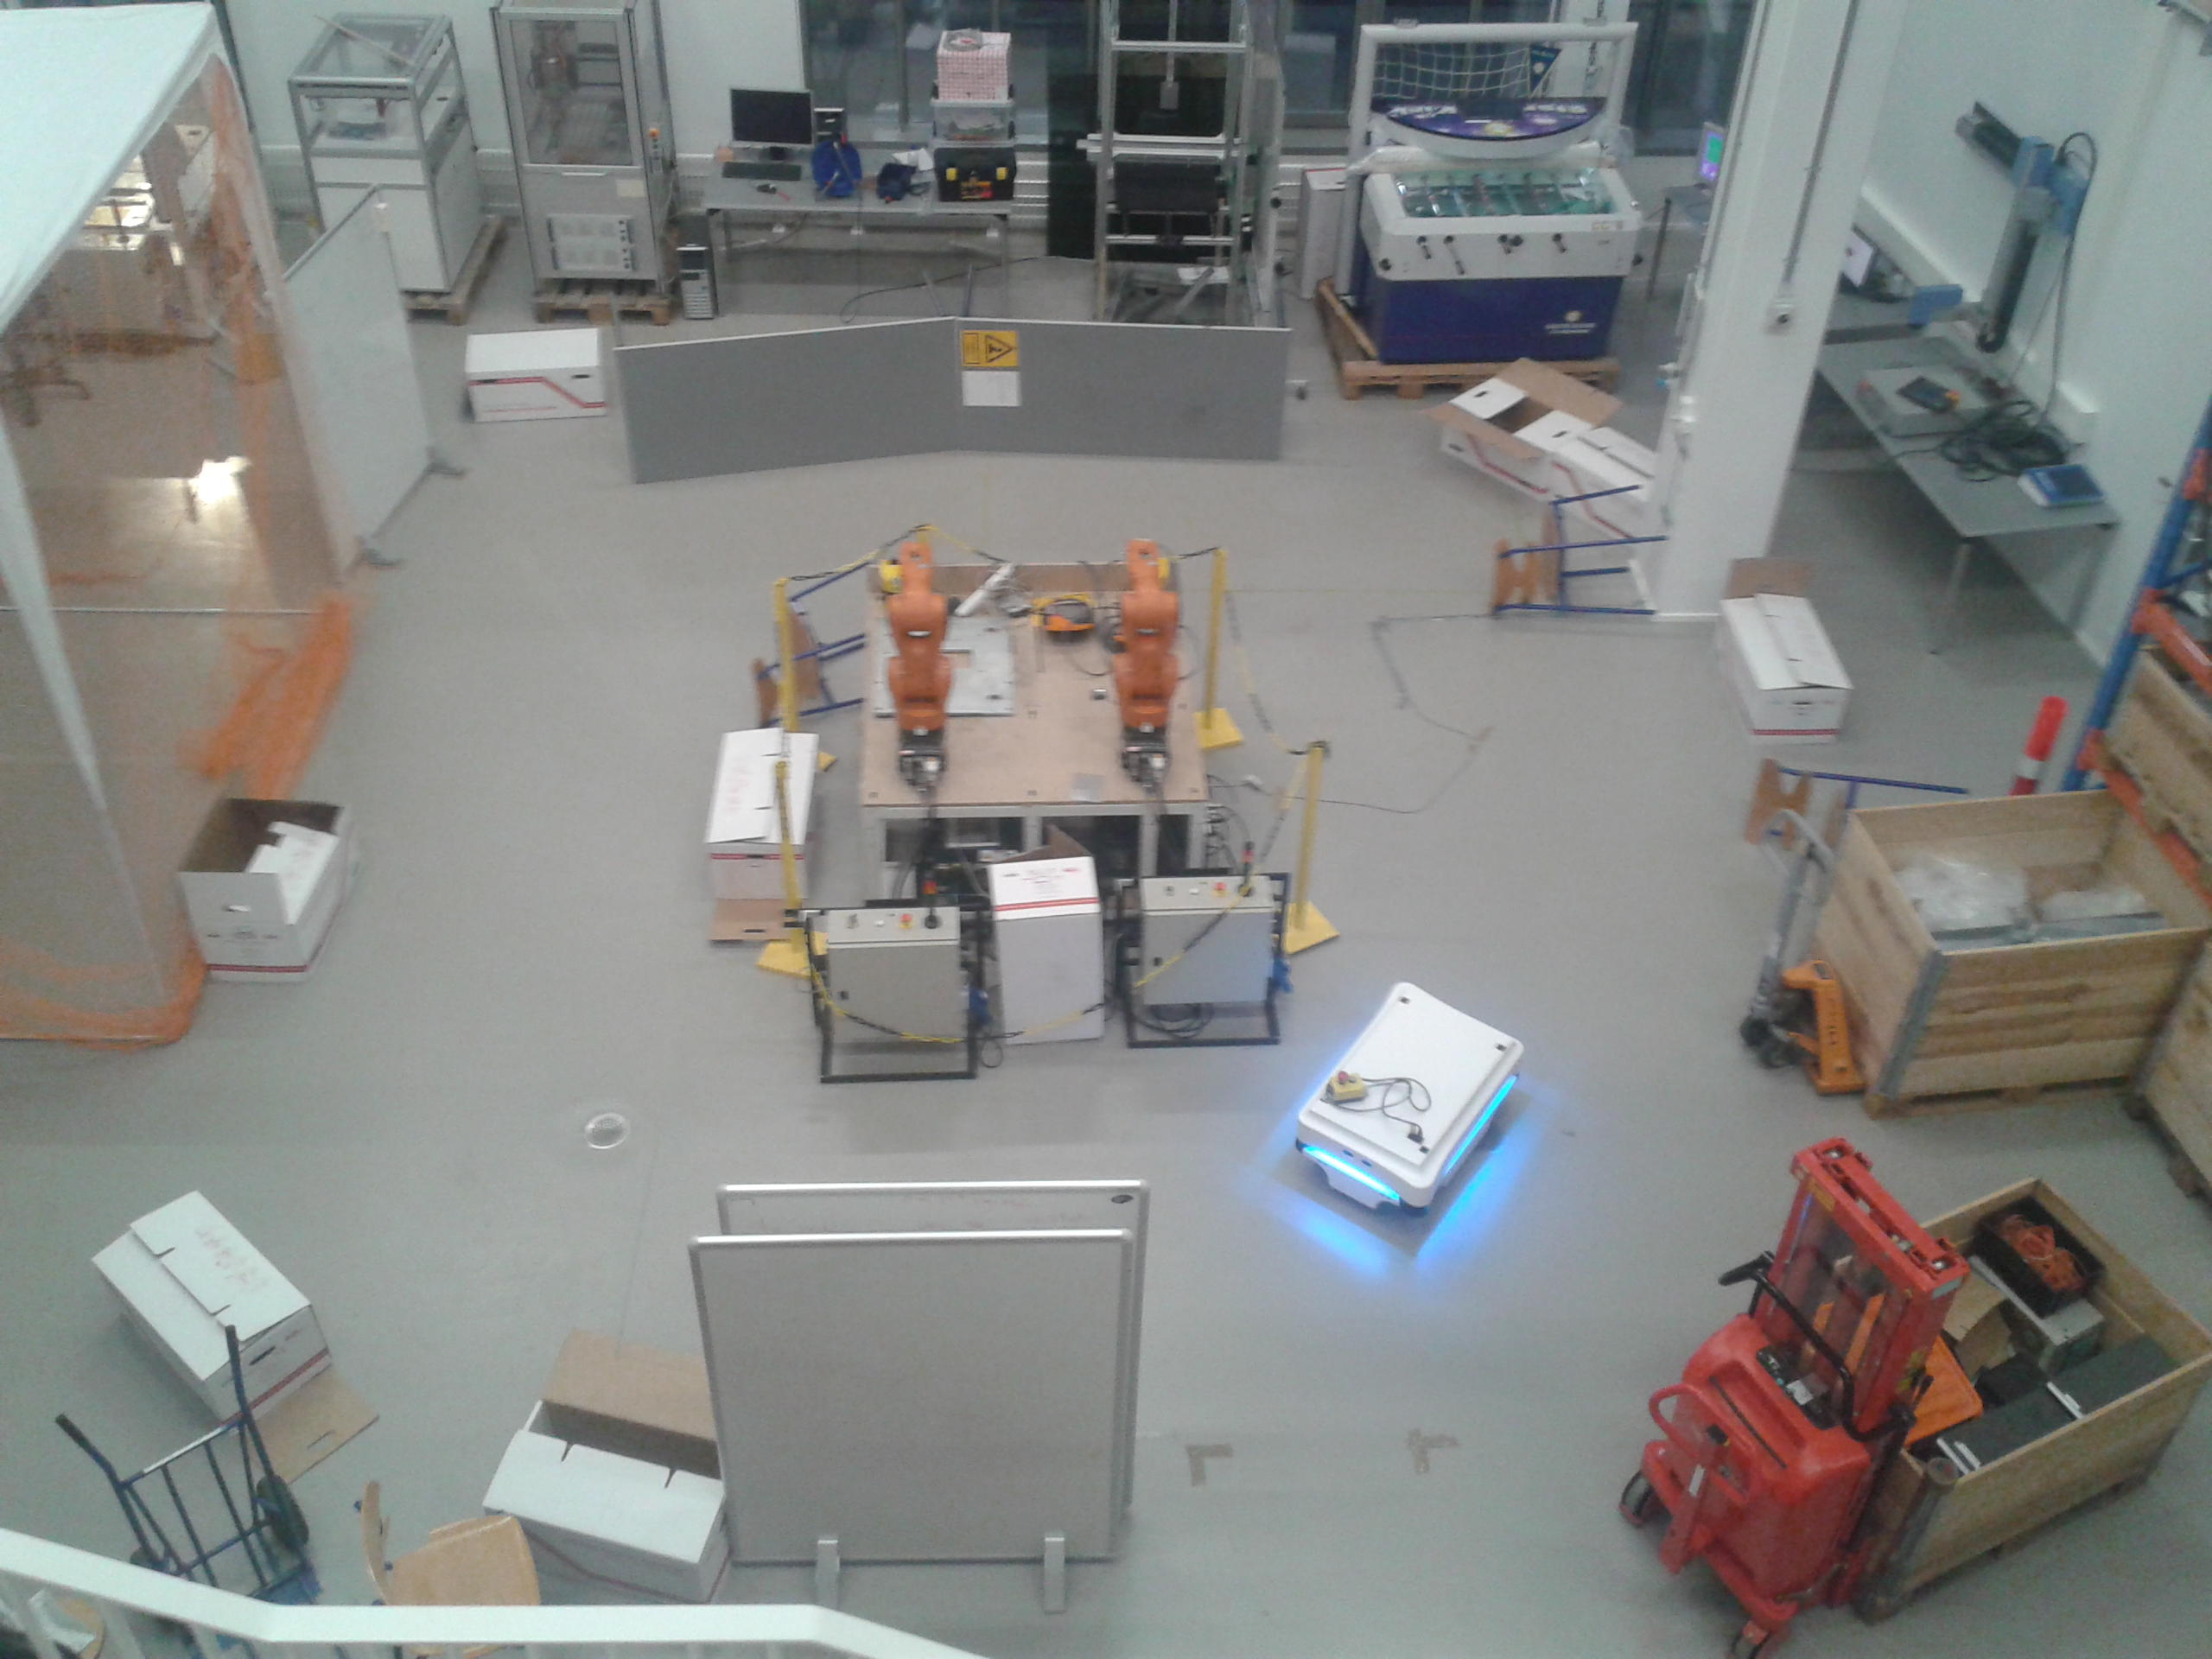
\includegraphics[width=1\textwidth]{chapters/evaluation/figures/mayhem_robolab4}
		\caption{Fourth environment}
		\label{fig:location_environment4}
	\end{subfigure}
	\caption{Robolab at SDU technical college with different positions of obstacles.}
	\label{fig:robolab_mayhem}
\end{figure}

In the first environment shown in figure \ref{fig:location_environment1} a table was tilted, eight cardboard boxes and a whiteboard was placed. 
In the second environment shown in figure \ref{fig:location_environment2}, two of the boxes was moved closer, one more table and whiteboard was flipped, and a pallet was moved. 
In the third environments \ref{fig:location_environment3} even more changes are introduced in the form of tilted chairs and a pallet. 
In the forth environment shown in figure \ref{fig:location_environment4} some of the boxes are moved and a whiteboard is moved out of sight. 
This results in fewer changes to the environment since the map was created than in the third environment.

\subsection{Estimation Uncertainty with Dynamic Map Representation}
During navigation the covariance and robot pose, estimated by AMCL is logged. 
The covariances in positions are ignored here to keep the data analysis simple while still enabling a comparison of the estimations achieved while using a static- and dynamic map.
\todo{Bad argument}

Figure \ref{fig:location_data_angle} shows the estimated standard deviation on the estimated orientation of the robot while navigating with a static- and dynamic map representation in the four different environments.
It shows that the estimation variates less when using a dynamic map representation.
In the first environment the estimated deviation is mostly smaller when using a dynamic map representation, but during a short time of every cycle of moving around the obstacle, it is much larger. 
While the lowest estimated deviation while using a static map is only slightly higher in the other environments, it is still occasionally very large, whereas it remains rather constant while using a dynamic map representation. 
From figure \ref{fig:location_data_hist_angle} it is evident that the estimation is distributed with a normal distribution.
The one-sided student-T test with unequal variance shows that the estimated standard deviation of the orientation is smaller when using a dynamic map with $p < 0.001$.

\begin{figure}[htbp]
	\begin{subfigure}[t]{1\textwidth}	
		\centering	
		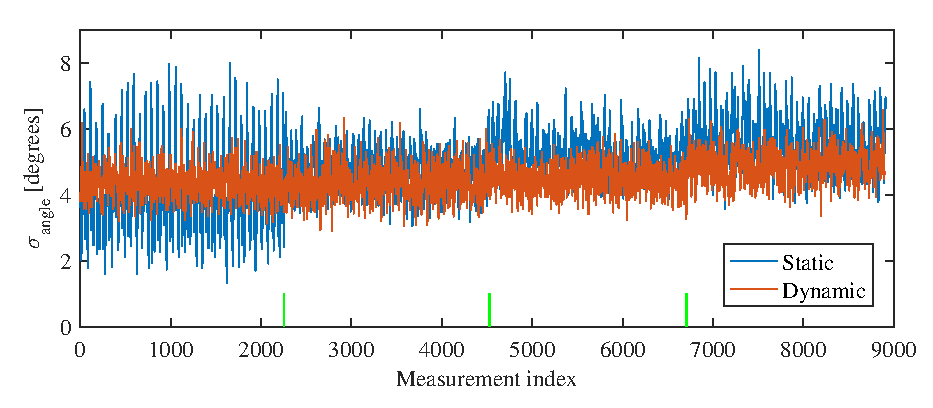
\includegraphics[scale=1.0]{chapters/evaluation/figures/location_data_angle}
		\caption{Estimated standard deviation on the estimated orientation during the four different experiments. The green lines in the figure indicates changes from one experiment to the next.}
		\label{fig:location_data_angle}
	\end{subfigure}
	\begin{subfigure}[t]{1\textwidth}
		\centering
		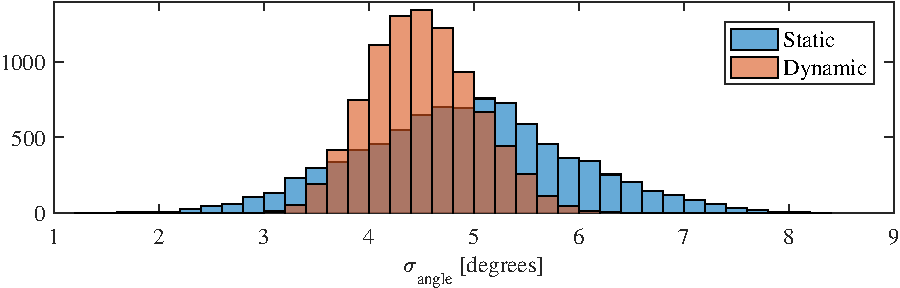
\includegraphics[scale=1.0]{chapters/evaluation/figures/location_data_hist_angle-crop}
		\caption{Histogram of the estimated standard deviation of the orientation estimate.}
		\label{fig:location_data_hist_angle}
	\end{subfigure}
	\caption{Estimated standard deviation of the estimated orientation while navigating in the four different environments.}
	\label{fig:location_angle_evaluation}
\end{figure}

Figure \ref{fig:location_data_x} and \ref{fig:location_data_y} shows the estimated standard deviation of the estimated x- and y position receptively, while navigating with a static- and dynamic map in the four different environments. 
It is clear that the estimated deviation varies less when using a dynamic map representation.
Where the estimated deviation remains almost constant throughout the four experiments, it is often much larger when using a static map representation. 
These tendencies are especially profound in the last environment in the x direction and in the first in the y direction. 
The estimations are not normal distributed as seen in figure \ref{fig:location_data_hist_x} and \ref{fig:location_data_hist_y}.
While the histograms over the position deviations indicates that the estimated deviation is smaller when using a dynamic map representation the median of it is not statistical significant smaller. This is evident from the one-sided Wilcoxon Rang-Sum test.
\begin{figure}[htbp]
	\begin{subfigure}[t]{1\textwidth}	
		\centering	
		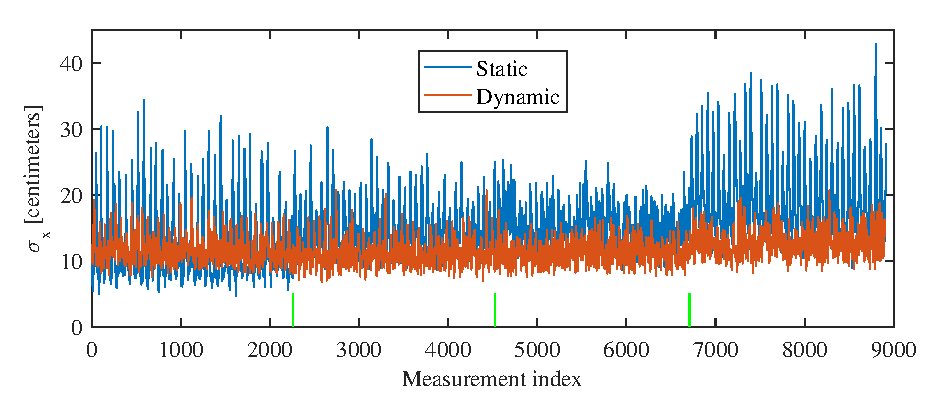
\includegraphics[scale=1.0]{chapters/evaluation/figures/location_data_x}	
		\caption{Estimated standard deviation on the estimated x-position during the four different experiments. The green lines in the figure indicates changes from one experiment to the next.}
		\label{fig:location_data_x}
	\end{subfigure}
	
	\begin{subfigure}[t]{1\textwidth}
		\centering
		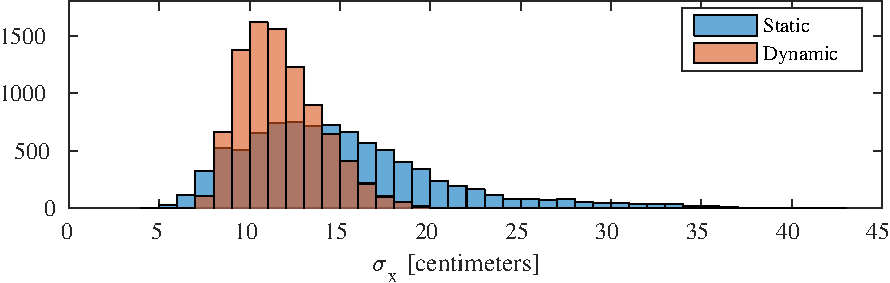
\includegraphics[scale=1.0]{chapters/evaluation/figures/location_data_hist_x-crop}
		\caption{Histogram of the estimated standard deviation of the x-position estimate.}
		\label{fig:location_data_hist_x}
	\end{subfigure}
	\caption{Estimated standard deviation of the estimated x-position while navigating in the four different environments.}
	\label{fig:location_x_evaluation}
\end{figure}

\begin{figure}[htbp]
	\begin{subfigure}[t]{1\textwidth}	
		\centering	
		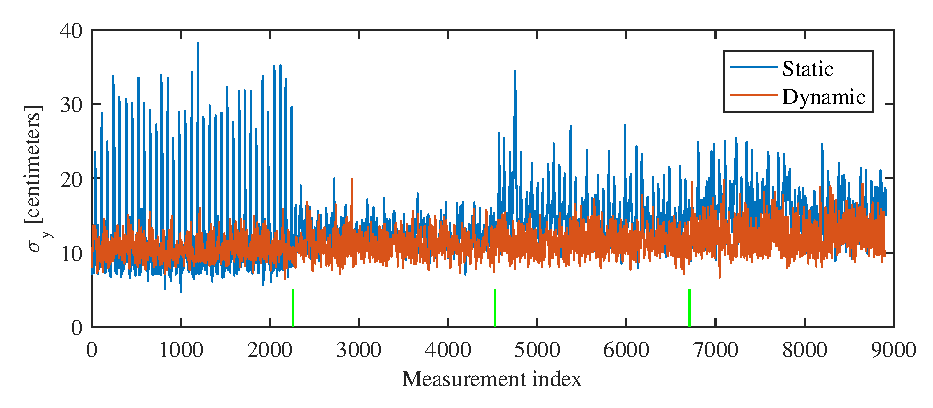
\includegraphics[scale=1.0]{chapters/evaluation/figures/location_data_y}	
		\caption{Estimated standard deviation on the estimated y-position during the four different experiments. The green lines in the figure indicates changes from one experiment to the next.}
		\label{fig:location_data_y}
	\end{subfigure}
	
	\begin{subfigure}[t]{1\textwidth}
		\centering
		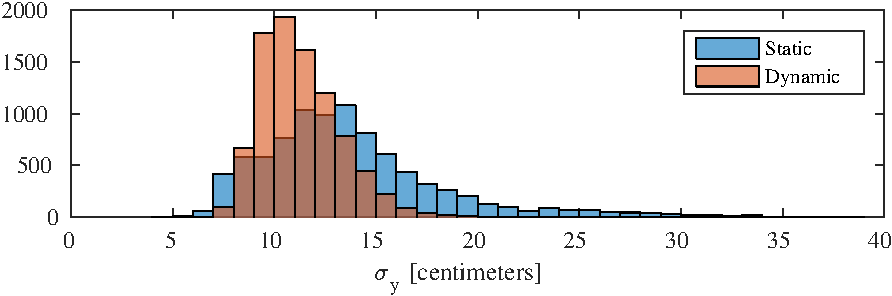
\includegraphics[scale=1.0]{chapters/evaluation/figures/location_data_hist_y-crop}
		\caption{Histogram of the estimated standard deviation of the y-position estimate.}
		\label{fig:location_data_hist_y}
	\end{subfigure}
	\caption{Estimated standard deviation of the estimated y-position while navigating in the four different environments.}
	\label{fig:location_y_evaluation}
\end{figure}

\subsection{Jumps in Position Estimation with Dynamic Map Representation}
The AMCL localizations with a static map makes large jumps between estimated localization when the robot is located close to the box standing by the net furthest from the camera in figure \ref{fig:robolab_mayhem}. 
In all four environments the estimated position suddenly jumps to be much closer to the net. 
The effect is probably due to multiple consecutive laser scans hitting the boxes, but scoring the particles as if they had hit the net behind them.
Figure \ref{fig:amcl_covariance_static1} shows this jump in the estimated position of the robot superimposed on the map as it is observed by the robot.
Considering that the robot cannot physically be located so close to the boxes, the correct robot pose is more closely estimated with the dynamic map representation as shown in figure \ref{fig:amcl_covariance_dynamic1}.
The estimated robot pose is superimposed on the dynamic map representation used by AMCL.

\begin{figure}[htbp]
	\centering
	\begin{subfigure}[t]{0.45\linewidth}
		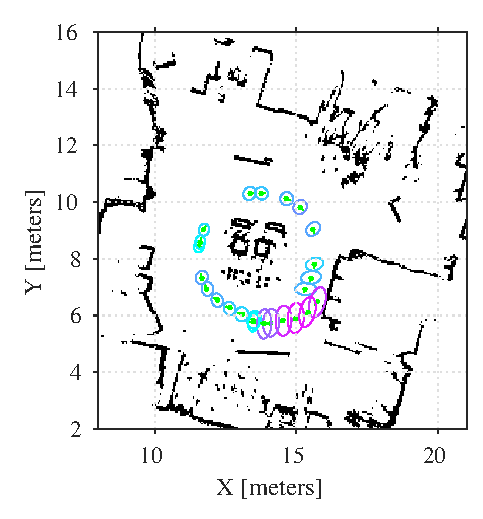
\includegraphics[width=\linewidth]{chapters/evaluation/figures/localization_static_map1}
       	\caption{Static map in the first test.}
        \label{fig:amcl_covariance_static1}
	\end{subfigure}
    \hspace{2mm}
   	\begin{subfigure}[t]{0.45\linewidth}
        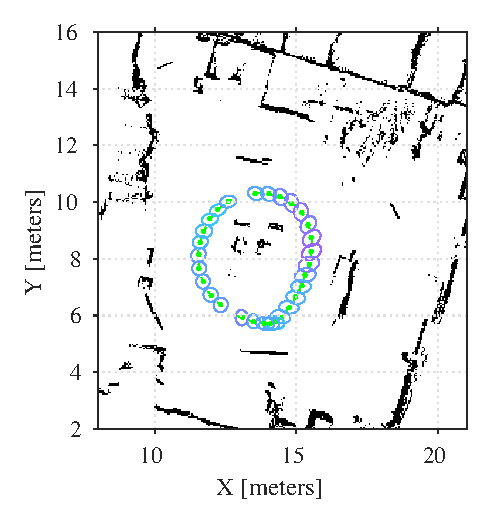
\includegraphics[width=\linewidth]{chapters/evaluation/figures/localization_dynamic_map1}
       	\caption{Dynamic map in the first test.}
    \end{subfigure}
   	\begin{subfigure}[t]{0.45\linewidth}
        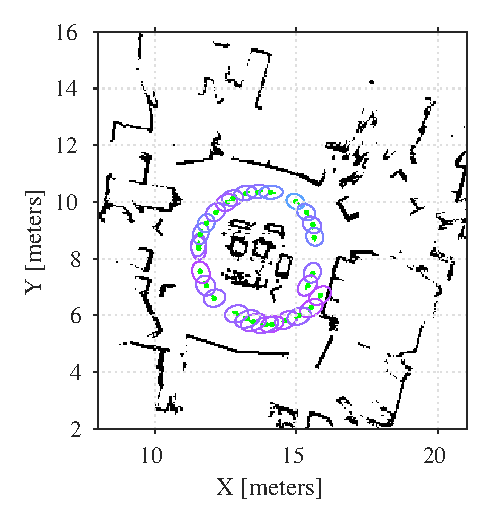
\includegraphics[width=1\linewidth]{chapters/evaluation/figures/localization_static_map3}	
        \caption{Static map in the third test.}
    \end{subfigure}
    \hspace{2mm}
   	\begin{subfigure}[t]{0.45\linewidth}
        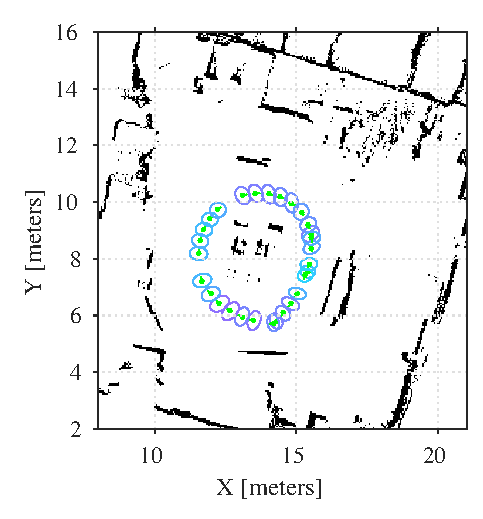
\includegraphics[width=\linewidth]{chapters/evaluation/figures/localization_dynamic_map3}
        \caption{Dynamic map in the third test.}
    \end{subfigure}
    
	\begin{subfigure}[t]{1.0\linewidth}
        \centering
        \hspace{9mm}
		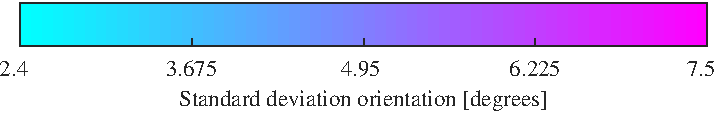
\includegraphics[scale=1]{chapters/evaluation/figures/precision_bar-crop}
	\end{subfigure}
   	\caption{Covariances estimated by AMCL with static and dynamic map representations shown with contours marking one standard deviation around the robot's estimated pose(green).}
\end{figure}

The estimated deviation is generally higher in the third environment where fewer of the laser scans match with the static map representation as shown in figure \ref{fig:amcl_covariance_dynamic1}. 
The reason for the fewer matches is that the dynamic obstacles block for the light beams. 
When using the dynamic map representation shown in figure \ref{fig:amcl_covariance_static3} the estimated deviation is smaller, since the obstacles that has consistently been present while navigating with the dynamic map in the first and second environment.

By comparing the maps in figure  \ref{fig:amcl_covariance_static1} and \ref{fig:amcl_covariance_static3} it is evident that only the obstacles that was present in the first environment is considered static enough to be included in the dynamic map in figure \ref{fig:amcl_covariance_dynamic3}.

